\section{Systemudvikling}
	\begin{frame}
		\frametitle{Objektorienteret Analyse \& Design}
		\textbf{Hovedaktiviteter}
			\begin{itemize}
				\item Systemvalg
				\item Analyse af problemområde
				\item Analyse af anvendelsesområde
				\item Design af arkitektur
			\end{itemize}
	\end{frame}
		
	\begin{frame}
		\frametitle{Systemvalg - Systemdefinition}
		\begin{center}
    		\begin{tabular}{ | l | p{5cm} |} \hline
   				\textbf{Kriterie:} & \bf{Beskrivelse:} \\ \hline
    			\textbf{B}etingelser & Ulønnede udviklere. \\ \hline
    			\textbf{A}nvendelsesområde & Brugerne og deres computere. \\ \hline
    			\textbf{T}eknologier & Internetforbindelse. PC. Tablet. Mobiltelefon. \\ \hline
    			\textbf{O}bjekter & Opskrifter. Ingredienser. \\ \hline
    			\textbf{F}unktioner & Søgningsværktøj. Find opskrifter indeholdende valgte ingredienser \\ \hline
    			\textbf{F}ilosofi & Folk smider mad ud, fordi de mangler et sted at bruge deres rester. \\ \hline
    		\end{tabular}
		\end{center}
	\end{frame}
	
	% Hændelsestabel
	\begin{frame}
		\frametitle{Analyse af Problemområde - Hændelsestabel}
		\begin{itemize}
			\item Madrester og madlavning i de danske husstande
		\end{itemize}
		\begin{center}
    		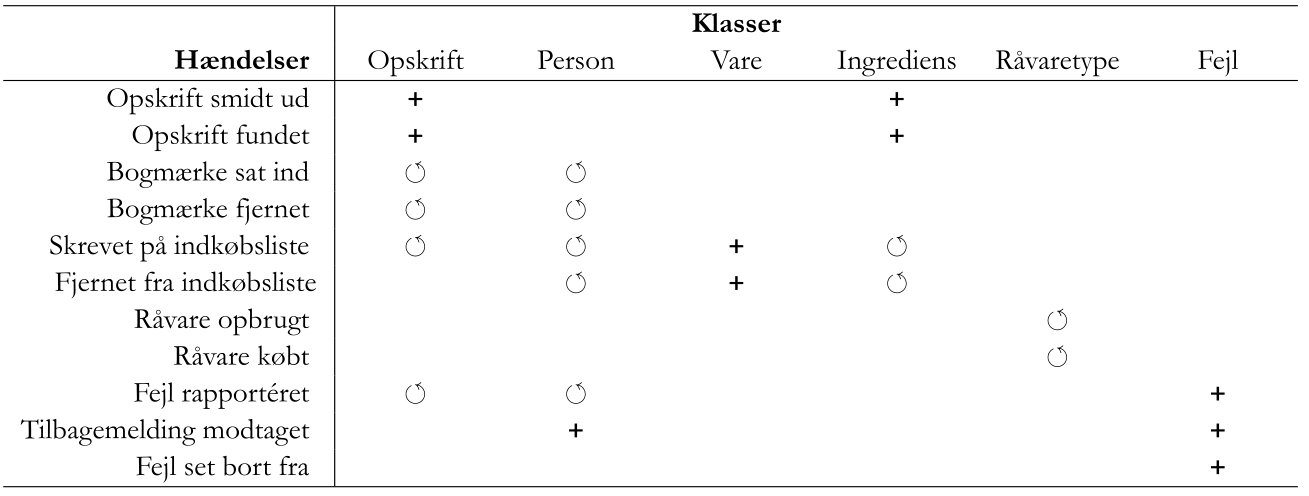
\includegraphics[scale=0.3]{billeder/haendelsestabel.png}
		\end{center}
	\end{frame}
	
	% Aktørtabel
	\begin{frame}
		\frametitle{Analyse af Anvendelsesområde - Aktørtabel}
		\begin{itemize}
			\item Brugerne og deres computere
			\item Fastlægge kravene til brugen 
		\end{itemize}
		\begin{center}
    		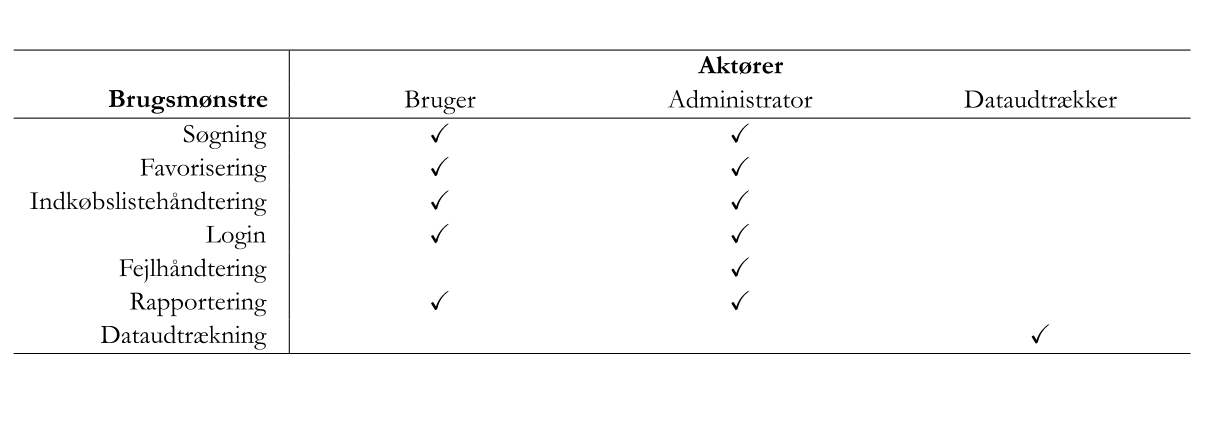
\includegraphics[scale=0.35]{billeder/aktoertabel.png}
		\end{center}
	\end{frame}
	
	% Kriterietabel
	\begin{frame}
		\frametitle{Design af Arkitektur - Kriterietabel}
		\begin{itemize}
			\item At strukturere et system
		\end{itemize}
		\begin{center}
    		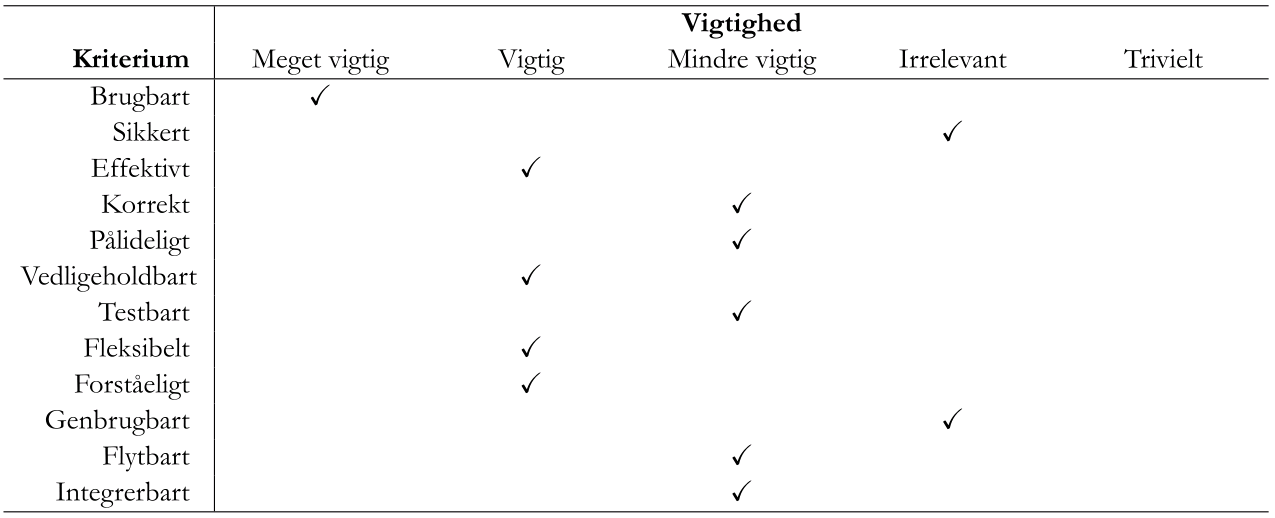
\includegraphics[scale=0.3]{billeder/kriterietabel.png}
		\end{center}
	\end{frame}